% Figura -- Comparacion de modelos en P1. Version en espanol.
% -------------------------------------------------------------------------
% GENERADO POR _figura_comparacion.py DEL REPOSITORIO MIGRA-IA.
% NO EDITAR A MANO: cualquier cambio se pierde al regenerar.
% Las cifras del trivial y del clasico salen de correr _baseline.py; la de la
% propuesta, de data/figura_comparacion_propuesta.csv.
%
% PAQUETES NECESARIOS EN EL PREAMBULO DEL .tex PRINCIPAL:
%   \usepackage{pgfplots}      NUEVO
%   \pgfplotsset{compat=1.18}  NUEVO
%   \usepackage[table]{xcolor} ya esta (Tabla I)
%
% ESTADO: MODO DISENO: la propuesta aun no esta medida; su barra va como hueco.
% -------------------------------------------------------------------------
\definecolor{migrapropuesta}{HTML}{1F4E9C}
\begin{figure}[!tb]
\centering
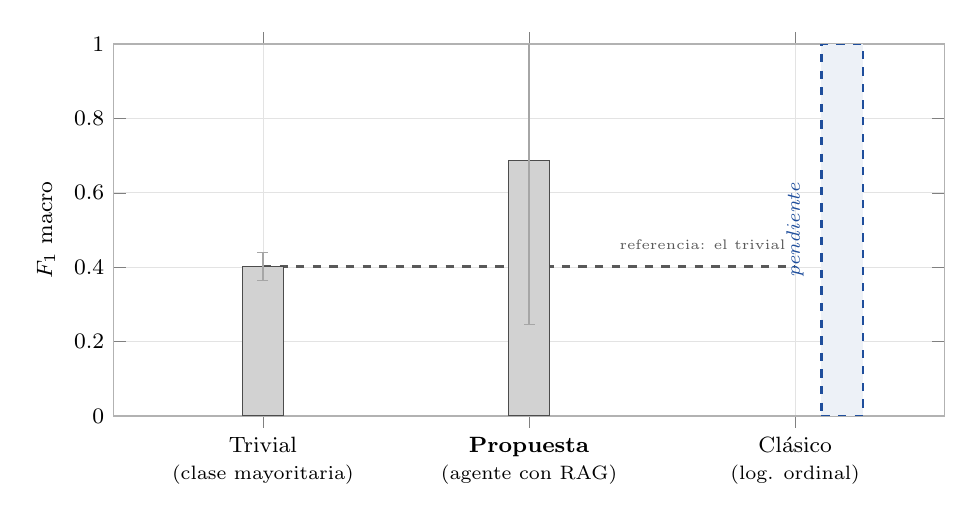
\begin{tikzpicture}
\begin{axis}[
  ybar,
  width=\columnwidth,
  height=0.52\columnwidth,
  bar width=15pt,
  ymin=0, ymax=1.0,
  ytick={0,0.2,0.4,0.6,0.8,1.0},
  ylabel={$F_1$ macro},
  symbolic x coords={trivial,clasico,propuesta},
  xtick=data,
  xticklabels={Trivial\\\scriptsize(clase mayoritaria), Clásico\\\scriptsize(log. ordinal), \textbf{Propuesta}\\\scriptsize(agente con RAG)},
  xticklabel style={align=center, font=\footnotesize},
  tick label style={font=\footnotesize},
  label style={font=\footnotesize},
  enlarge x limits=0.28,
  grid=major,
  grid style={gray!22, line width=0.3pt},
  axis line style={gray!60},
  error bars/error bar style={gray!70, line width=0.6pt},
]

% --- Linea de referencia: el modelo trivial ------------------------------
\addplot[sharp plot, dashed, black!65, line width=0.8pt, forget plot]
  coordinates {(trivial,0.402) (propuesta,0.402)};
\node[anchor=south east, font=\tiny, text=black!65]
  at (axis cs:propuesta,0.422) {referencia: el trivial};

% --- Los dos modelos de referencia, en gris ------------------------------
\addplot+[ybar, draw=black!70, fill=gray!35, error bars/.cd,
          y dir=both, y explicit]
  coordinates {
    (trivial,0.402) +- (0,0.038)
    (clasico,0.688) +- (0,0.442)
  };

% --- La propuesta: hueco marcado, no hay medida todavia ------------------
\addplot[ybar, draw=migrapropuesta, line width=1pt, dashed,
         fill=migrapropuesta!8, forget plot]
  coordinates {(propuesta,1.0)};
\node[rotate=90, font=\scriptsize\itshape, text=migrapropuesta]
  at (axis cs:propuesta,0.5) {pendiente};

\end{axis}
\end{tikzpicture}
\caption{Comparación de modelos en el subproblema P1 (riesgo ordinal), sobre la misma partición estratificada y agrupada por fabricante ($n=9$, $k=2$). La métrica es el $F_1$ macro, la que decide; la línea discontinua marca el valor del modelo trivial, por debajo del cual no hay resultado publicable. Las barras de error son la desviación entre pliegues: se solapan, de modo que la ventaja del modelo clásico es indicio de que la antigüedad lleva señal y no evidencia de que el modelo funcione. La barra de la propuesta, en color, queda vacía hasta medirla bajo esa misma partición.}
\label{fig:comparacion}
\end{figure}
